\scanpage{129}
\deleted{
\deleted{Proposition}
\margin{passer au N$^\circ$ \unsure{précédent}}
\figure{\begin{tikzpicture}\draw[->](0,0)..controls(-.8,1)and(-.8,2)..(.6,2.8);\draw(1,2.6)--(1.5,1.8)--(2.8,2.6);\draw(1.5,1.8)circle(.06);\end{tikzpicture}}

(i) Si $A=k[t_{\unsure{1|0}},-,t_n]_{\mathfrak m}$, $\mathfrak m$ maximal, $k$ un corps alors \deleted{$\dim A=n\quad A$ est de dim} \inserted{$A$ est \uline{régulier}, de dim $n$} $\dim A=n$
\margin{\deleted{$A[t_1--t_n]$}}

\uline{Dem.} Par \unsure{chgt} de base, on est \unsure{ramené} au cas où $k(\mathfrak m)=k$, on a alors une \deleted{\unsure{régulière de}} \inserted{$A$-suite} \deleted{paramètres} de $n$ éléments engendrant l'idéal maximal $\mathfrak m$

\margin{\deleted{\unsure{(ii)}} \uline{Cor}}
$A$ anneau \inserted{local} noeth. Alors pour tt idéal maximal $M$ de $B=A[t_1-t_n]$ induisant $M\cap A=\mathfrak m$, on a
\[
\dim B_M=\dim A+n
\]
\uline{Cor} si $A$ \unsure{anneau local} noeth, $\dim A[t_1,-,t_n]=\dim A+n$

\uline{Cor} Utilisons la formule des dimensions dans le cas des algèbres de type fini sur $k$. [\unsure{résulte du} lemme de normalisation] on trouve, si $M$ induit $\mathfrak m$
\[
\dim B_M=\dim A+\underbrace{n-\deg\operatorname{tr}\ k(M)/k(\mathfrak m)}_{\nu=\dim[ B_M\otimes_A k=k[t_1,-t_n]_M ]}
\]
\deleted{\uline{Cor} $A$ anneau noeth. Alors $\dim A[t_1,-t_n]=\dim A+n$}

\deleted{(ii) Si $A=k[t_1,-t_n]_{\mathfrak m}$, $\mathfrak m$ maximal, $k$ un corps, \unsure{Alors} $A$ \unsure{est}}
\figure{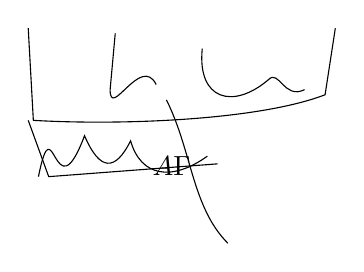
\begin{tikzpicture}[x=.65cm,y=.65cm]
\draw(0,3.6)--(.1,1.8)..controls(1.8,1.7)and(4.5,1.8)..(5.8,2.3)--(6,3.6);
\draw(3.4,3.2)..controls(3.3,2.2)and(4,2)..(4.7,2.6)..controls(4.9,2.8)and(5,2.2)..(5.4,2.4);
\draw(1.7,3.5)--(1.6,2.4)..controls(1.6,1.8)and(2.2,3.1)..(2.5,2.5);
\draw(0,1.8)--(.4,.7)--(3.7,.95);\draw(.2,.7)..controls(.5,2.2)and(.5,-.1)..(1.1,1.5)..controls(1.4,.8)and(1.7,.8)..(2,1.4)..controls(2.2,.7)and(2.8,.6)..(3.5,1.1);
\node at(2.8,.9){$\unsure{A\Gamma}$};
\draw(2.7,2.2)..controls(3.2,1.2)and(3.2,.1)..(3.9,-.6);
\end{tikzpicture}}
\uline{Dem.} \deleted{\unsure{Prof}}
\[
\left\{\begin{array}{l}
\operatorname{prof}B_M=\operatorname{prof}A+\nu\\[1ex]
\operatorname{coprof}\unsure{B_M|\Phi_M}=\operatorname{coprof}A-
\end{array}\right.
\]

\uline{Cor.} $X=Y[t_1-t_n]$, $Y$ loc. noeth. \unsure{soit $x\in X$}, $y\in Y$. Soit P l'une des propriétés\ldots\ldots. Alors $X$ est P \unsure{en $x$} si $Y$ est \unsure{''|``}\unsure{en $y$}.
\unsure{(Montrer} \unsure{pour} \unsure{certaines} propriétés).
\figure{\begin{tikzpicture}\draw(0,0)--(0,2.2);\end{tikzpicture}}
}
\mspage{128}

